
\documentclass[journal,transmag]{IEEEtran}
\hyphenation{op-tical net-works semi-conduc-tor}

\usepackage{enumitem}

% *** GRAPHICS RELATED PACKAGES ***
%
\ifCLASSINFOpdf
   \usepackage[pdftex]{graphicx}
  % declare the path(s) where your graphic files are
  % \graphicspath{{../pdf/}{../jpeg/}}
  % and their extensions so you won't have to specify these with
  % every instance of \includegraphics
  % \DeclareGraphicsExtensions{.pdf,.jpeg,.png}
\else
  % or other class option (dvipsone, dvipdf, if not using dvips). graphicx
  % will default to the driver specified in the system graphics.cfg if no
  % driver is specified.
  % \usepackage[dvips]{graphicx}
  % declare the path(s) where your graphic files are
  % \graphicspath{{../eps/}}
  % and their extensions so you won't have to specify these with
  % every instance of \includegraphics
  % \DeclareGraphicsExtensions{.eps}
\fi
% graphicx was written by David Carlisle and Sebastian Rahtz. It is
% required if you want graphics, photos, etc. graphicx.sty is already
% installed on most LaTeX systems. The latest version and documentation
% can be obtained at: 
% http://www.ctan.org/pkg/graphicx
% Another good source of documentation is "Using Imported Graphics in
% LaTeX2e" by Keith Reckdahl which can be found at:
% http://www.ctan.org/pkg/epslatex
%
% latex, and pdflatex in dvi mode, support graphics in encapsulated
% postscript (.eps) format. pdflatex in pdf mode supports graphics
% in .pdf, .jpeg, .png and .mps (metapost) formats. Users should ensure
% that all non-photo figures use a vector format (.eps, .pdf, .mps) and
% not a bitmapped formats (.jpeg, .png). The IEEE frowns on bitmapped formats
% which can result in "jaggedy"/blurry rendering of lines and letters as
% well as large increases in file sizes.
%
% You can find documentation about the pdfTeX application at:
% http://www.tug.org/applications/pdftex





\begin{document}

\title{\textsc{Caracterización molecular y anotación funcional de una proteína hipotética (GenBank: CAI46211.1) de \textit{Homo sapiens}}.}

\author{
\IEEEauthorblockN{Molecular characterization and Functional annotation}
\IEEEauthorblockA{Pontificia Universidad Javeriana, Bogotá, Colombia}
\IEEEauthorblockA{ Laura Echeverri, Paula Ugueto, William Gómez}

}
% The paper headers
\markboth{ BIOINFORMÁTICA. Noviembre 18~2022. }%
{Shell \MakeLowercase{\textit{et al.}}: Bare Demo of IEEEtran.cls for IEEE Transactions on Magnetics Journals}
\IEEEtitleabstractindextext{%

	\begin{abstract}
		A pesar de los esfuerzos colectivos de muchos científicos que tratan de comprender el cerebro humano, y los efectos del cáncer y la formación de tumores malignos en este, para disminuir la gran tasa de mortalidad que ocurre a nivel mundial por estas causas, aún hace falta mucho por entender, descubrir y analizar para estar más cerca de solucionar estas enfermedades. Es por esto que avances en las investigaciones en la caracterización molecular y anotación funcional de las proteínas del cerebro que se secuencian en estudios de cáncer a través del mundo, es necesario para mejorar nuestra comprensión del cáncer. Por lo tanto, el presente artículo busca revelar las funciones de una proteína hipotética de Homo sapiens hallada en estudios del Proyecto del Genoma Alemán (GenBank CAI46211.1, UniProt Q5JV90). Se utilizaron diferentes herramientas bioinformáticas para predecir la función, ubicación y propiedades físico-químicas para encontrar funciones de unión a quinasas tipo C, actividad transductora, así como 4 motivos claramente identificados: DUF3544, Bromodominio, PHD, y PWWP. Además, se estudió la estructura tridimensional de la proteína y se consiguió una cobertura excelente para un 33\% de la proteína. Por último, se identificó que el dominio DUF3544 se encuentra aún funcionalmente sin caracterizar y puede representar una oportunidad de investigar y descubrir nuevos conocimientos.  

	\end{abstract}
	\begin{IEEEkeywords}
	Proteína hipotética, Análisis bioinformático, Tejido cerebral, C-quinasa, Homo Sapiens.
	 	\end{IEEEkeywords}}


\maketitle
\IEEEdisplaynontitleabstractindextext
\IEEEpeerreviewmaketitle


\section{Introducción}

Con el fin de analizar una proteína no caracterizada haciendo uso de herramientas bioinformáticas se buscó en la base de datos de proteínas de NCBI una proteína hipotética que fuera de nuestro interés para hacer una caracterización molecular y anotación funcional de esta proteína, con el fin de identificar su función, ubicación, familia, estructura, dominios, motivos principales y sus sitios activos.  Se encontró entonces en un estudio sobre cáncer una proteína hipotética (CAI46211) cuya secuencia ha sido identificada como potencialmente involucrada con los procesos de metástasis.

Esta proteína hipotética fue secuenciada por el Centro de Investigación Alemán de Cáncer junto con la Universidad Ludwig Maximilians en el marco del Proyecto del Genoma Alemán [1]. El principal autor de esta secuenciación es el Profesor Dr. Stefan Wiemann, que ha enfocado sus trabajos en el cáncer de seno. El cáncer, así como muchas otras enfermedades humanas nace de aberraciones genéticas que pueden ser heredadas o pueden ocurrir espontáneamente en células somáticas. Estos defectos causan actividades anormales en los productos de genes y provocan funcionamientos erróneos en interacciones moleculares y celulares, terminando en tumores y progreso del cáncer. El objetivo central de esta unidad de investigación es entender la complejidad de los mecanismos moleculares en la regulación de redes de señalamiento y cómo esto impacta en el desarrollo del cáncer, metástasis y la resistencia a las drogas. Para esto se hacen proyectos a gran escala, usando tecnologías genómicas y proteómicas para analizar diferentes genes y proteínas candidatos a influenciar en el tema. Por medio de estos análisis se construye conocimiento que se explota posteriormente para la identificación de nuevos marcadores para diagnóstico y pronóstico, así como para desarrollar estrategias de intervención terapéutica. Es así como el estudio de estas proteínas hipotéticas da luces sobre aquellas que están involucradas en los procesos de metástasis y cáncer de mama, estudiando sus actividades intrínsecas y sus redes con otras proteínas o genes. 

Los estudios han demostrado que las redes proteicas asociadas a tumores cancerígenos son complejas y que involucran diferentes tipos de células [1]. Se puede, por lo tanto, estudiar sobre el impacto que tienen perturbaciones individuales a diferentes niveles (ADN, ARN, proteínas, metabolitos, fenotipos) en una gran variedad de vías celulares. Con esto se busca tener un mejor entendimiento de la conectividad entre sistemas de interacción en múltiples capas. 

Actualmente, de la proteína hipotética CAI46211 se sabe que tiene una longitud de 934 aminoácidos y que se encuentra en el ser humano (\textit{Homo sapiens}). El tejido en el que fue hallada es el cerebral y en etapa de desarrollo fetal. Está altamente relacionada, como veremos a lo largo de este artículo, con una proteína quinasa de unión tipo C. Es decir, hace parte de una familia de proteínas quinasas enzimas (PKC) involucradas en controlar la función de otras proteínas por medio de la fosforilación de los grupos hidroxilos en los residuos de aminoácidos serina y treonina en estas proteínas. Es así como se sabe que las enzimas PKC juegan un papel importante en numerosas cascadas de señales de transducción.  Por lo tanto, en este artículo se realizó la caracterización molecular y anotación funcional de una proteína hipotética encontrada en NCBI utilizando diferentes herramientas bioinformáticas.

\section{Métodos}
 \subsection{\textbf{ Obtención de la secuencia e identificación de similitudes}}

 La secuencia de la proteína hipotética fue tomada de la base de datos de NCBI. Se descargó en formato FASTA para poder cargarla en diferentes plataformas que nos acerquen a su caracterización in silico. El primer paso para inferir la función de esta proteína fue buscar similitudes con las herramientas del NCBI, se corrió un BLAST ( $https://blast.ncbi.nlm.nih.gov/Blast.cgi$ ) para identificar similitudes. 
 
 \subsection{\textbf{ Alineamiento múltiple de secuencias y análisis filogenético}}

Se implementó MUSCLE ($https://www.ebi.ac.uk/Tools/msa/muscle/ $), herramienta del servidor EBI para hacer un análisis comparativo entre nuestra proteína hipotética y cinco proteínas homólogas para determinar el grado de similitud entre estas. Adicionalmente con Phylogeny.fr ($http://www.phylogeny.fr/ $) se realizó el análisis filogenético. 

\subsection{\textbf{ Análisis de propiedades fisicoquímicas}}

Se determinaron las propiedades fisicoquímicas de la proteína por medio de la plataforma ProtParam ($https://web.expasy.org/protparam/$), una herramienta que suministra Expasy ($https://www.expasy.org/$). Estas incluyen el peso molecular, el pI teórico, los principales aminoácidos que la componen, su composición atómica, la media vida estimada, su índice de inestabilidad y su índice alifático, el número total de residuos cargados negativa y positivamente y las predicciones de GRAVY ($https://www.gravy-calculator.de/$) . 


\subsection{\textbf{ Análisis de ubicación subcelular}}
Se utilizó DeepLoc ($http://deeploc.cs.uni-freiburg.de/$) para predecir su ubicación, esta parece ser el núcleo. Los resultados se validaron con WoLFPSORT ($https://www.genscript.com/wolf-psort.html$), que arrojó como segunda opción de ubicación citosol-núcleo. 

\subsection{\textbf{ Dominios conservados, motivos, identificación de familia y superfamilia}}

Se corrió la secuencia de la proteína para encontrar en el banco del NCBI algún dominio conservado que pueda indicar las funciones principales de la proteína, así como la familia y superfamilia a la que puede pertenecer. Adicionalmente, se buscó en MOTIF de GenomeNet ($https://www.genome.jp/$) los motivos identificables en la proteína y utilizando InterPro ($https://www.ebi.ac.uk/interpro/$) se identificaron sus términos de Gene Onthogoly ($http://geneontology.org/$), confirmaron presencia de dominios conservados y familias homólogas. 

\subsection{\textbf{ Predicción de estructuras secundarias}}

La plataforma de PSIPRED ($http://bioinf.cs.ucl.ac.uk/psipred/$) nos permitió visualizar la estructura que conforma cada uno de los aminoácidos de la proteína. Del mismo modo, SOPMA ($https://npsa-prabi.ibcp.fr/cgi-bin/npsa_automat.pl?page=npsa\%20_sopma.html$) arroja información sobre las proporciones de estructuras que se tienen en base a la cantidad de aminoácidos que las conforman. 

\subsection{\textbf{ Predicción de la estructura tridimensional}}

Al haber hallado en las herramientas previas homologías entre esta proteína hipotética y otras, se utilizó el programa Swiss Model ($https://swissmodel.expasy.org/$) para predecir su estructura tridimensional. Sin embargo, al no obtener un modelamiento total de la proteína, se recurrió a otras herramientas como Alphafold ($https://alphafold.com/$) y Phyre2 ($http://www.sbg.bio.ic.ac.uk$).

\subsection{\textbf{ Evaluación de la calidad del modelo}}

La evaluación de los modelos tridimensionales predichos por Swiss Model, Alphafold y Phyre2 se evaluó en PROCHECK ($https://www.ebi.ac.uk/thornton-srv/software/PROCHECK/$) y en Verify3D ($https://www.doe-mbi.ucla.edu/verify3d/$). 

\subsection{\textbf{ Detección de sitios activos}}

A pesar de la falta de información sobre la estructura tridimensional de la proteína hipotética, se utilizó el programa CASTp ($http://sts.bioe.uic.edu/castp/index.html?2was$) para identificar los sitios activos de la estructura que se conoce. 


\section{Resultados y Discusión}
El flujograma del estudio se muestra en la Figura 1
	\begin{figure}[!h]
		\center
		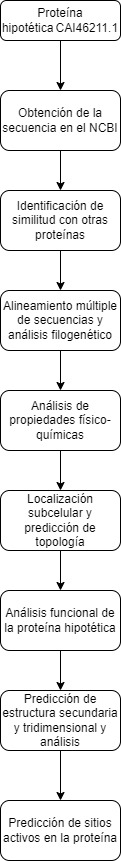
\includegraphics[width=2cm]{imagenes/flujograma.png}
		\caption{Flujograma del trabajo}
		\label{1}
	\end{figure}

\subsection{\textbf{ Secuencia e información de similitudes}}

Después de correr el Blastp, se encontraron más de 100 resultados con un porcentaje de similitud elevado. En los parametros del algoritmo de Blastp no se especificó ningún filtro en cuanto a organismos y se observa que los resultados se encuentran además en primates, incluyendo algunas proteínas caracterizadas del Homo Sapiens. Los resultados que mayor porcentaje de identidad tienen (hasta un 99.56\%) son aquellos de proteínas quinasas C; las variaciones se tienen de acuerdo con las distintas isoformas y los distintos organismos portadores. En la Figura 2 se observan las proteínas con alto nivel de similitud en forma de árbol. 
\begin{figure}[!h]
	\center
	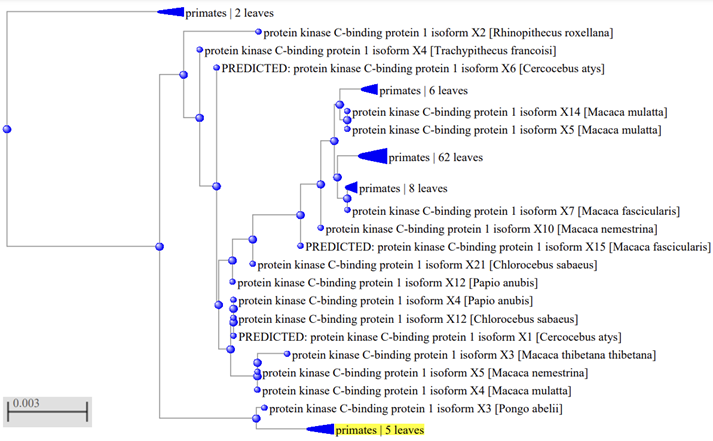
\includegraphics[width=8.5cm]{imagenes/similitudes.png}
	\caption{Árbol con resultados de proteínas similares a la proteína hipotética en cuestión arrojados por Blastp}
	\label{2}
\end{figure}

Por otro lado, se halla con Blastp la mayor identidad con proteína de union a quinasa C, isoforma $CRA_e$ del organismo \textit{Homo sapiens}, donde no fue necesario abrir ningún gap y solo se observan 4 mutaciones. En la Tabla 1 a continuación se observan las similitudes más significativas de alineamiento con otras proteínas.  

\begin{table}[!h]
	\begin{tabular}{|l|l|l|l|l|l|}
	\hline
	Descripción& Organismo & \begin{tabular}[c]{@{}l@{}}Query \\cover\end{tabular}
	& \begin{tabular}[c]{@{}l@{}}E \\value\end{tabular} & \begin{tabular}[c]{@{}l@{}}\% \\identity \end{tabular}
	&  \begin{tabular}[c]{@{}l@{}}Access \\(NCBI)\end{tabular} \\ \hline
	\begin{tabular}[c]{@{}l@{}}protein \\kinase\\C-binding \\protein 1\\isoform \\$CRA_e $\end{tabular}    & \begin{tabular}[c]{@{}l@{}}Homo \\sapiens\end{tabular}&97\%  &0.0   &99.56\%   &\begin{tabular}[c]{@{}l@{}}EAW\\75707.1   \end{tabular}\\ \hline
	\begin{tabular}[c]{@{}l@{}}protein \\kinase\\C-binding \\protein 1\\isoform \\$CRA_k$\end{tabular}   &\begin{tabular}[c]{@{}l@{}}Homo \\sapiens\end{tabular} &97\%   &0.0   &99.56\%   &\begin{tabular}[c]{@{}l@{}}EAW\\75714.1  \end{tabular}\\ \hline
	\begin{tabular}[c]{@{}l@{}}protein \\kinase\\C-binding \\protein 1\\isoform X7\end{tabular}   &\begin{tabular}[c]{@{}l@{}}Pan \\troglodytes \end{tabular}&92\%   &0.0   &96.18\%   &\begin{tabular}[c]{@{}l@{}}XP\_016\\793551.2   \end{tabular}\\ \hline
	\begin{tabular}[c]{@{}l@{}}protein \\kinase\\C-binding \\protein 1\\isoform X3\end{tabular}   &\begin{tabular}[c]{@{}l@{}}Pongo \\abelii \end{tabular}&92\%   &0.0   &95.96\%  &\begin{tabular}[c]{@{}l@{}}XP\_024\\094347.1   \end{tabular}\\ \hline
	\begin{tabular}[c]{@{}l@{}}protein \\kinase\\C-binding \\protein 1\\isoform X3\end{tabular}   & \begin{tabular}[c]{@{}l@{}}Macaca \\thibetana \end{tabular}&92\%   &0.0   &95.17\%   &\begin{tabular}[c]{@{}l@{}}XP\_050\\601089.1  \end{tabular}\\ \hline
	\end{tabular}
	\caption{Resultados de similitud arrojados por el Blastp }
\end{table}

\subsection{\textbf{ Alineamiento múltiple de secuencias y análisis filogenético}}
Se utilizó MUSCLE para hacer un alineamiento múltiple entre la secuencia hipotética y 5 proteínas homologas descubiertas con Blastp y calcular el grado de similitud entre estas 6 proteínas, como se observa en la Tabla , se ve el nivel de similitud en una matriz de identidad.

\begin{table}[htb]
	\begin{tabular}{|lllllll|}
	\hline
	\multicolumn{7}{|l|}{\begin{tabular}[c]{@{}l@{}}Identity matrix of the hypothetical protein\\ $( tr| Q5JV90|Q5JV90\_HUMAN)$and its 5  most homologous proteins  \end{tabular}}        \\ \hline
	\multicolumn{1}{|l|}{\begin{tabular}[c]{@{}l@{}} XP\_024\\094347.1  \end{tabular}} &100.00  &99.03  &93.42  &91.64   &93.36   &93.79  \\ \cline{1-1}
	\multicolumn{1}{|l|}{\begin{tabular}[c]{@{}l@{}} XP\_050\\601089.1	\end{tabular}} &99.03  &100.00   &92.69   & 91.00  &92.61  &93.04   \\ \cline{1-1}
	\multicolumn{1}{|l|}{\begin{tabular}[c]{@{}l@{}} XP\_016\\793551.2 \end{tabular}}&93.42  &92.69   &100.00   &91.85   &93.58  &94.00   \\ \cline{1-1}
	\multicolumn{1}{|l|}{\begin{tabular}[c]{@{}l@{}} EAW\\75714.1 \end{tabular}}&91.64   &91.00   &91.85   &100.00   &97.53   &97.86   \\ \cline{1-1}
	\multicolumn{1}{|l|}{\begin{tabular}[c]{@{}l@{}} tr|Q5JV90\\|Q5JV90\\\_HUMAN \end{tabular}}&93.36   &92.61  &93.58  &97.53   &100.00   &99.57   \\ \cline{1-1}
	\multicolumn{1}{|l|}{\begin{tabular}[c]{@{}l@{}} EAW\\75707.1 \end{tabular}} &93.79  &93.04   &94.00   &97.86   &99.57   &100.00   \\ \hline
	\end{tabular}
	\caption{Matriz de identidad para la proteína hipotética en cuestión. }
	\end{table}

	Con esta tabla de identidad confirmamos el grado de similitud de nuestra proteína hipotética frente a las proteínas homólogas encontradas. Se toma particularmente la proteína EAW75707.1, al ser esta una proteína NO-hipotética, como punto de comparación para dilucidar más acerca de la estructura de CAI46211.1 . 

	Para hace el análisis filogenético se utilizó la herramienta Phylogeny.fr la cual nos muestra una relación evolutiva entre estas 6 proteínas que se están comparando como se observa en la Figura 3.

	
\begin{figure}[!h]
	\center
	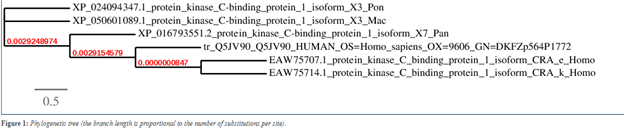
\includegraphics[width=8.5cm]{imagenes/arbol3.png}
	\caption{Árbol filogénico de proteína hipotética CAI46211.1}
	\label{3}
\end{figure}
Con la Figura 3 se valida la elección de la proteína EAW75707.1 como punto de comparación debido a su parentesco cercano. 


\subsection{\textbf{ Características fisicoquímicas}}
La proteína de estudio tiene 934 aminoácidos y su peso molecular es de 103 962 Da. Su punto isoeléctrico calculado es de 8.45, es decir básico. Esto se debe a un exceso de aminoácidos básicos como lo son la arginina, lisina o la histidina. Efectivamente, esto se puede observar en la Tabla 3: 

\begin{table}[htb]
	\begin{tabular}{|l|l|l|}
	\hline
	 AA& Cantidad  &Porcentaje  \\ \hline
	 Ser (S) & 101  & 10.8\%  \\ \hline
	 Lys (K) & 90  & 9.6\%  \\ \hline
	 Pro (P) & 77  & 8.2\%  \\ \hline
	 Glu (E) & 66  & 7.1\%  \\ \hline
	 Thr (T) & 61  & 6.5\%  \\ \hline
	\end{tabular}
	\caption{Distribución de aminoácidos en la proteína hipotética.  }
	\end{table}
	El número total de residuos cargados negativamente (Asp + Glu) y positivamente (Arg + Lys) resultaron ser 113 y 122 respectivamente. Su índice de inestabilidad resultó ser de 59.49, clasificando esta proteína como inestable y su índice alifático de 59.49, relativamente bajo, por lo que se infiere que su temperatura tampoco es estable a altas temperaturas. Por otro lado, su GRAVY (Grand average of hydropathicity) es de e-0.701, lo que indica que esta proteína es apolar. Finalmente, su media vida estimada es de 30 horas in vitro y en mammalian reticulocytes, superior a 20 horas in vivo en yeast y superior a 10 horas in vivo en escherichia coli. 
	Se calculó también que posee 14502 átomos, repartidos entre carbonos, hidrógenos, nitrógenos, oxígenos y sulfuros. Su fórmula química es $C_{4567} H_{7207} N_{1259} O_{1425} S_{44}$ . 
	

\subsection{\textbf{ Anotación funcional de la proteína hipotética}}

El resultado de InterPro Scan dice que pertenece a la Familia de proteínas de unión a proteína quinasa C. 
Los términos de GO que se obtienen allí son los siguientes:
Procesos Biológicos:

    • Regulación de la transcripción con plantilla de ADN (GO: 0006355)
Funciones Moleculares:

    • Unión a proteínas (GO:0005515)


Por otro lado, como se cuenta con un el registro de UniProt (Q5JV90) de esta proteína se han identificado 2 términos de GO:

    • Involucrada en la regulación de la transcripción con plantilla de ADN (GO: 0006355)

    • Permite la unión de iones metálicos (GO:0046872)

\subsection{\textbf{ Localización subcelular}}
Utilizando DeepLoc se predice con una probabilidad del 99.5\% que la proteína se ubica en el núcleo. Los resultados se muestran en la Figura 5 y concuerdan con lo reportado en UniProt.
\begin{figure}[!h]
	\center
	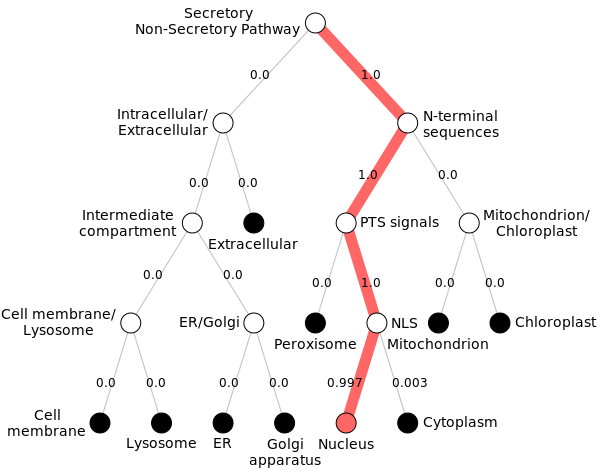
\includegraphics[width=8.5cm]{imagenes/localizacion.png}
	\caption{Ubicación celular de la proteína hipotética}
	\label{4}
\end{figure}

Utilizando WoLFPSORT se predice como ubicación el núcleo también y, como segunda opción, citosol-núcleo. Los resultados se observan en la Figura 5. 
\begin{figure}[!h]
	\center
	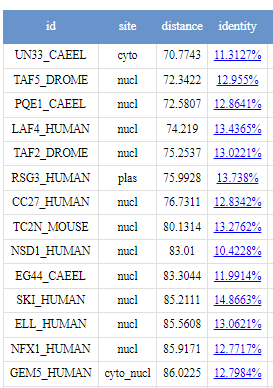
\includegraphics[width=7cm]{imagenes/loca.png}
	\caption{Localizacion celular de WoLFPSORT}
	\label{5}
\end{figure}


Utilizando LocTree3 obtenemos que la ubicación es en el núcleo y vemos un término de GO adicional, el que se observa en la Figura 6. 
\begin{figure}[!h]
	\center
	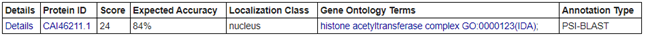
\includegraphics[width=8.5cm]{imagenes/loca2.png}
	\caption{Ubicacion celular de LocTree3}
	\label{6}
\end{figure}

\subsection{\textbf{ Dominios conservados, motivos, identificación de familia y superfamilia}}


Los resultados de los dominios conservados se pueden observar en la Figura 7 y se resumen en lo siguiente: DUF3544 (Domain of Unknown function), dominio de función desconocida encontrado en eucariotas. Este dominio tiene una longitud aproximada de 198 a 216 aminoácidos. El dominio suele encontrarse en las proteínas pfam00628, pfam01753, pfam00439 y pfam00855. En dónde la proteína analizada Pfam 12064 es la única perteneciente a la superfamilia cl3494.

\begin{figure}[!h]
	\center
	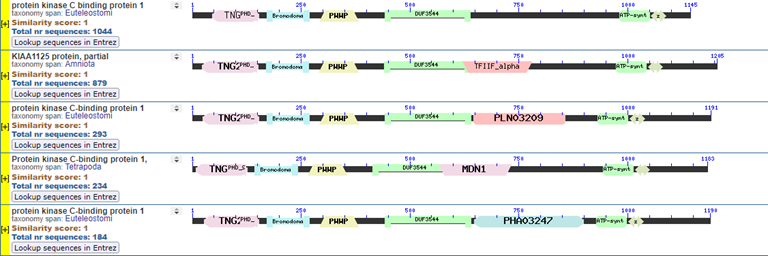
\includegraphics[width=10cm]{imagenes/dominios.png}
	\caption{Dominios conservados}
	\label{8}
\end{figure}

Podemos encontrar que el dominio DUF3544, así como el dominio PWWP, el dominio “PHD-finger” y el Bromodominio se presentan en varias proteínas identificadas principalmente como quinasas con unión tipo C. Estos motivos fueron encontrados también en MOTIFS Genome-Net en la posición 416-613 aa con un e-valor de 9.9e-97 para DUF3544 (PF12064), en la posición de 157-233 aa  con un e-valor de 8.6e-16 para el Bromodominio (PF00439), en la posición de 84-125 aa con un e-valor de 1.1e-06 para el dominio de PHD (PF00628), y en la posición de 274-343 aa con un e-valor de 3e-06 para el dominio PWWP (PF008559).  Motivos confirmados con las plataformas de InterPro y Pfam. 

\begin{figure}[!h]
	\center
	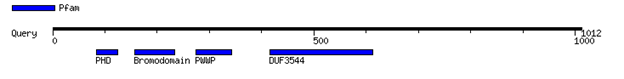
\includegraphics[width=8.5cm]{imagenes/motivos.png}
	\caption{Motivos con InterPro y Pfam}
	\label{9}
\end{figure}

Adicionalmente encontramos en InterPro que la proteína hipotética se relaciona con los términos GO de Proteína de unión (GO:0005515) como de regulación para transcripción (GO:0006355). Lo que coincide con su rol hipotético principal encontrado. 

\subsection{\textbf{ Análisis de estructura secundaria}}

Después de correr el PSIPRED, se obtuvo una predicción de la estructura secundaria de la proteína. Como se observa en la figura, sus aminoácidos se reparten entre strand, hélix y coil. No hay ninguna zona transmembranal ni tampoco de interacción con membranas. 

\begin{figure}[!h]
	\center
	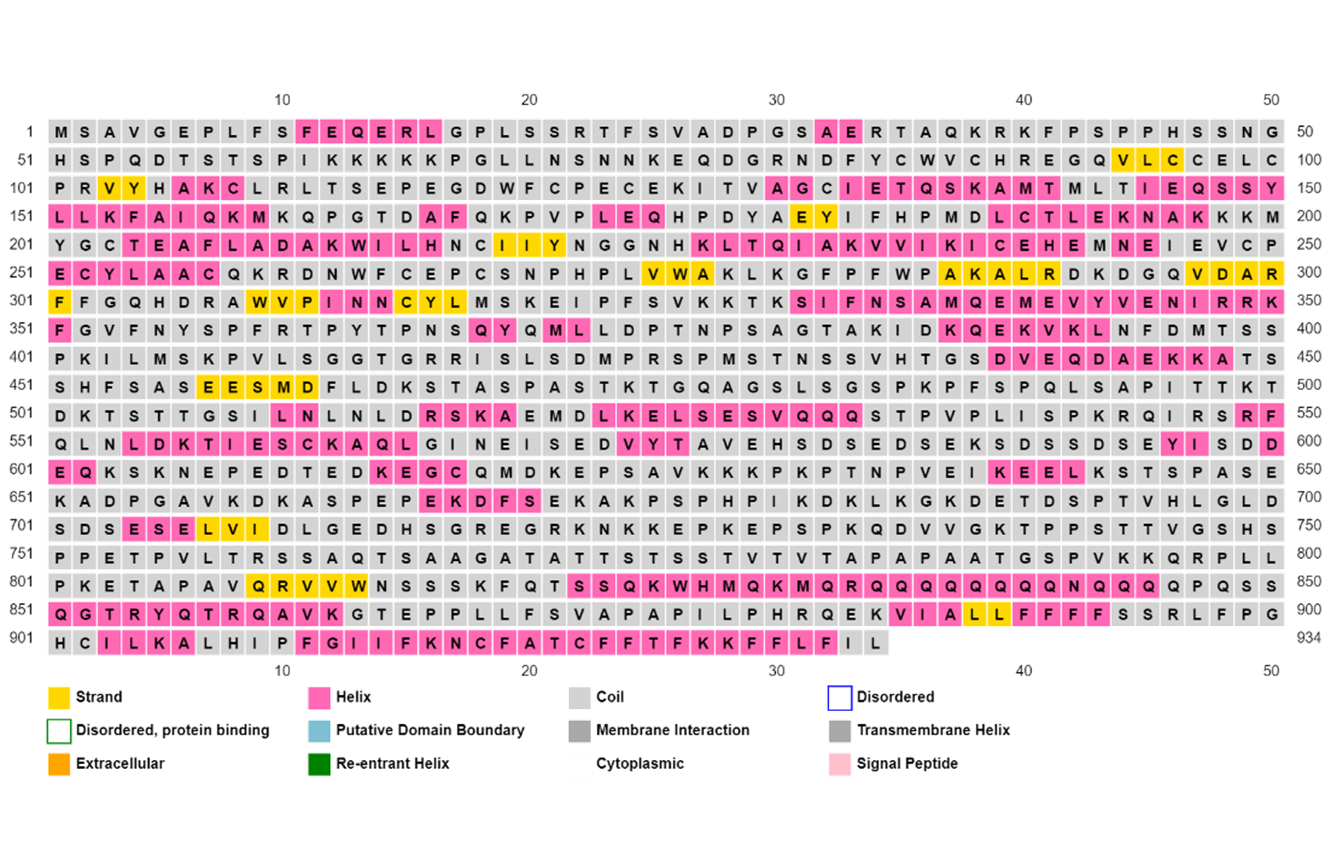
\includegraphics[width=8.5cm]{imagenes/secundaria.png}
	\caption{Configuración de los diferentes aminoácidos que conforman la proteína}
	\label{10}
\end{figure}

Las proporciones de estas configuraciones fueron halladas con SOPMA y se encuentran en la Tabla 4. 

\begin{table}[!h]
	\begin{tabular}{|l|l|l|}
	\hline
	Alpha Helix & 222 & 23.66\%  \\ \hline
	Extended strand & 129 & 13.81\%  \\ \hline
	Random coil& 555 & 59.42\%  \\ \hline
	Beta turn & 29 & 3.1\%  \\ \hline
	\end{tabular}
	\caption{Proporción de las configuraciones halladas en Figura 9. }
	\end{table}

\subsection{\textbf{ Análisis de la estructura tridimensional}}
Por otro lado, en Swiss Model se modeló la proteína en base a homologías. Los resultados fueron similares a los del BLASTp, pues la primera homología que se encontró fue con la Protein kinase C-binding protein 1 (código de acceso 5y1z.2.B) con una identidad del 99.07\%. 



\begin{figure}[!h]
	\center
	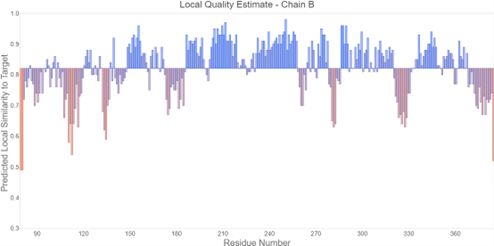
\includegraphics[width=8.5cm]{imagenes/barras.png}
	\caption{Similitud entre la Protein Kinase C-binding protein y la proteína hipotética en cuestión}
	\label{11}
\end{figure}

\begin{figure}[!h]
	\center
	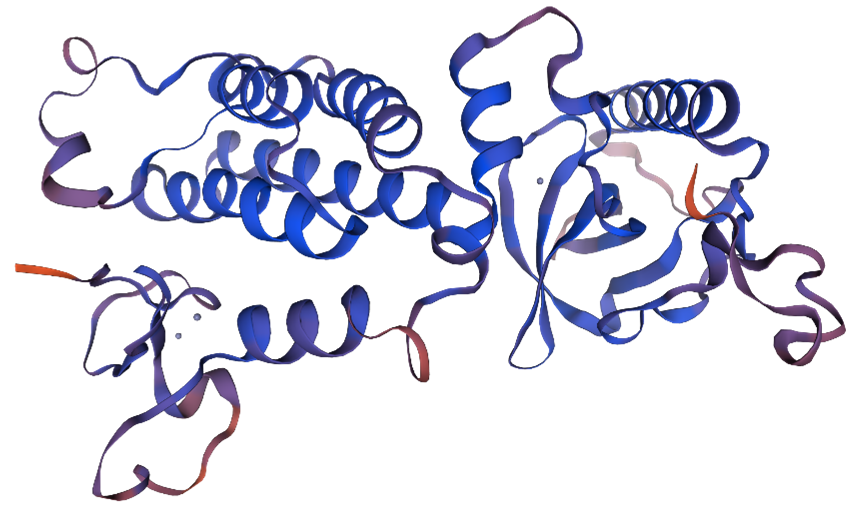
\includegraphics[width=8.5cm]{imagenes/swiss.png}
	\caption{Estructura tridimensional predicha en base a homologías}
	\label{12}
\end{figure}


En esta homología se encuentran las similitudes en cuanto a las hélices Alpha. Sin embargo, se observa que los extremos y algunas zonas no plegadas en forma de hélice difieren en cuanto al modelo elegido. Por lo mismo, el programa arroja otras dos homologías: Transcription intermediary factor 1-alpha (código de acceso 3o35.1.A) y bromodomain PHD finger transcription (código de acceso 2f6j.1.A). Con una identidad del 30.72\% y 25.47\% respectivamente.  

Sin embargo, se observa en la Figura 12 que una gran parte de la proteína no está modelada, puesto que no se encontraron homólogos que correspondieran a estas zonas. La línea verde es la secuencia de aminoácidos de la proteína hipotética, y toda la zona que no tiene azul por debajo es la que no fue modelada.  

\begin{figure}[!h]
	\center
	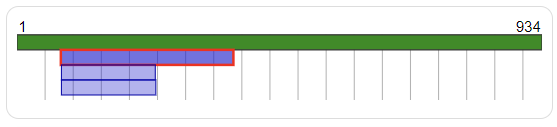
\includegraphics[width=8.5cm]{imagenes/alpha1.png}
	\caption{Parte modelada de la proteína por Swiss Model.}
	\label{13}
\end{figure}

El resultado que arroja AlphaFold para la estructura tridimensional de la proteína tienen niveles de certeza que corresponden a los resultados de Swiss Model.  


\begin{figure}[!h]
	\center
	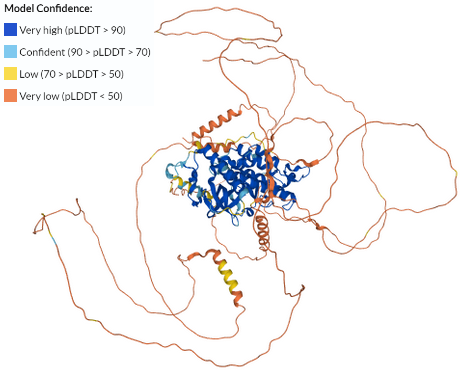
\includegraphics[width=8.5cm]{imagenes/alpha2.png}
	\caption{Modelo tridimensional de proteína hipotética en Alphafold.}
	\label{14}
\end{figure}

Como se observa en la Figura 13, las zonas de confianza alta son las mismas que aparecen en el modelo anterior, mientras que las de confianza muy baja son las que Swiss Model no modeló por falta de homologías.  

Para corroborar la estructura 3D de la proteína hipotéitca tambien se utilizó phyre2, 

El resultado de esta herramienta es el que se muestra en la imagen a continuación, y se reporta 100\% confidencia en una Cobertura del 33\% de la proteína. Además, se obtiene el tamaño en Armstrong de las dimensiones de la proteína.

\begin{figure}[!h]
	\center
	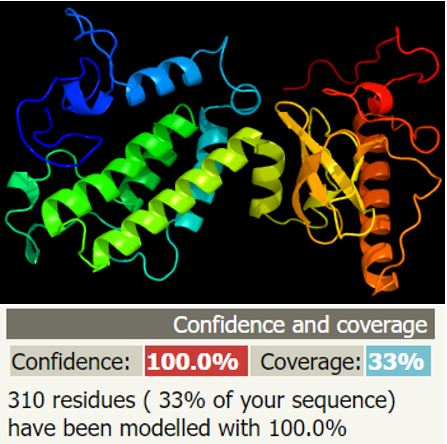
\includegraphics[width=6cm]{imagenes/phyre.JPG}
\caption{Puntajes del modelo tridimensional de Swiss Model de la proteína hipotética arrojados por Verify 3D. }
	\label{15}
\end{figure}


En PROCHECK y Verify3D se corroboraron los resultados del modelo obtenido con Alphafold, es decir el que predijo la estructura completa pero con un bajo porcentaje de confiabilidad en la mayor parte de la predicción, sin embargo, el resultado no fue positivo. Como se observa en la Figura 15, apenas 31.48\% de los residuos tuvieron un score 3D-1D superior o igual a 0.2. Como este porcentaje es inferior al 80\%, no se considera que sea un buen modelo. 
Por otro lado, PROCHECK arrojó los siguientes resultados: el valor del Ramachandran plot es del 64\%, por lo tanto, no alcanza   el porcentaje de un modelo válido. El 17.6\% de los residuos está en zonas permitidas, pero no muy favorables y el 13.9\% está en zonas no permitidas.
Estos resultados desfavorables de los modelos tridimensionales de la proteína se deben a que el modelo utilizado, el de Alphafold, tiene un gran porcentaje con una baja confiabilidad.  Debido a esto, se decidió correr los mismos programas, pero con el modelo de Swiss Model, que, a pesar de que represente únicamente el 33\% de la proteína hipotética en cuestión, tiene un alto grado de confiabilidad en este porcentaje. Los resultados se presentan en la Figura 15 y la Figura 16. 



\begin{figure}[!h]
	\center
	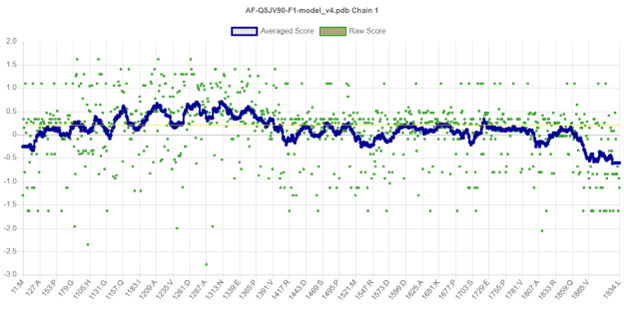
\includegraphics[width=8.5cm]{imagenes/procheck.png}
	\caption{Ramachandran plot para el modelo de Swiss Model de la proteína hipotética. }
	\label{16}
\end{figure}

\begin{figure}[!h]
	\center
	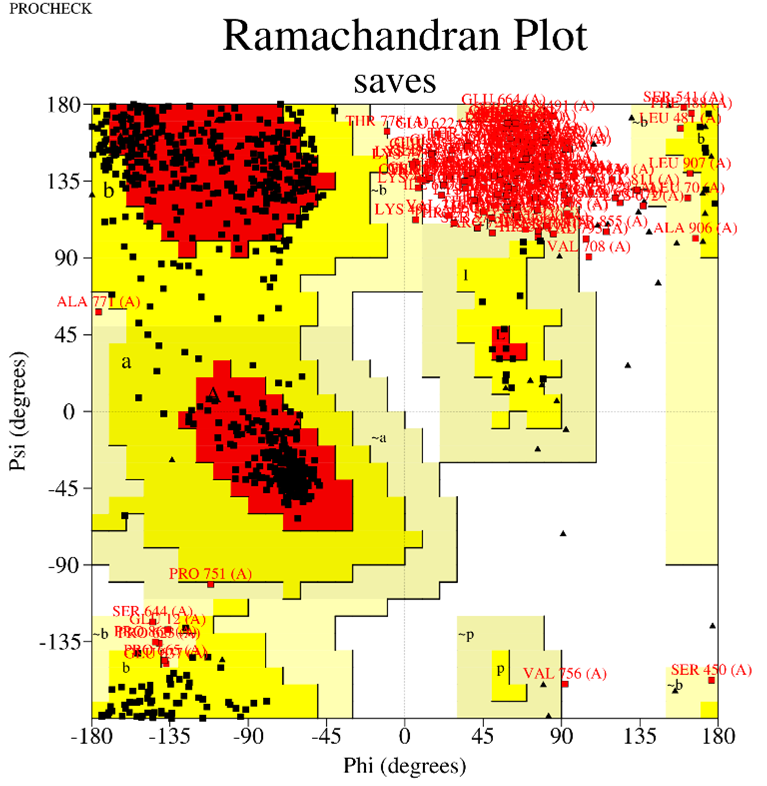
\includegraphics[width=6cm]{imagenes/ramachandran.png}
	\caption{Three-dimensional Phyre2 structure}
	\label{17}
\end{figure}
Como se observa en la Figura 15,  89.25\% de los residuos tienen un score 3D-1D superior o igual a 0.2. Al ser este un porcentaje superior al 80\%, se considera que el modelo predicho es un buen modelo. Por otro lado , en el Ramachandran plot presentado en la Figura 16  se observa que el 92.3\% de los residuos están ubicados en regiones muy favorables, 7.7\% en regiones permitidas y ningún porcentaje de los residuos se encuentran en zonas no permitidas. Por lo tanto, los 310 aminoácidos que fueron evaluados en cuanto a su estructura tridimensional tienen un alto grado de probabilidad de estar ubicados correctamente. 
Por lo tanto, el modelo de Alphafold es descartado por no pasar las pruebas de corroboración, y, por el contrario, el modelo de Swiss Model sí fue aprobado. A pesar de que este modelo nos dé un bajo porcentaje de la proteína hipotética, es información valiosa poder modelar correctamente ese porcentaje.
Se observa, además, al comparar con los dominios identificados en numerales anteriores, que en la región que se tiene bien modelada se encuentran los dominios DUF3544, Bromodominio, PHD y PWWP. 


\subsection{\textbf{ Análisis de la interacción proteína-proteína}}

Cuando se corrió STRING, arrojó una proteína con un 94,5\% de similitud: una proteína quinasa C-binding protein (código de acceso ZMYND8), que puede actuar como un correpresor transcripcional para KDM5D. Requerida para la regulación de diversos genes asociados con metástasis. Además, involucrada en la supresión de invasión celular en el cáncer de próstata. Por otro lado, contiene el bromodominio.    
Las interacciones halladas de esta proteína son las que se muestran en la Figura 17. 

\begin{figure}[!h]
	\center
	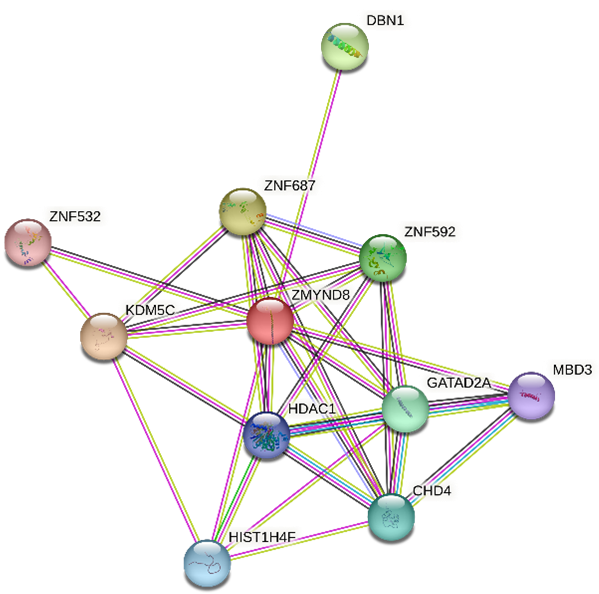
\includegraphics[width=6cm]{imagenes/interaccion.png}
	\caption{Interacciones de la proteína ZMYND8, homóloga a la proteína hipotética en cuestión. Verde: gen vecino, Rojo: Fusión de genes, Azul: gen con co-ocurrencia, Azul claro: información de bases de datos curadas, Fucsia: información determinada experimentalmente. }
	\label{18}
\end{figure}

En la Tabla 5 se describen las posibles funciones de las proteínas con las que interactúa la proteína homóloga a la proteína hipotética. 
	\begin{table}[]
		\begin{tabular}{|l|l|l|}
		\hline
		Protein  &Name  &Possible function    \\ \hline
		KDM5C& \begin{tabular}[c]{@{}l@{}}Desmetilasa 5C \\lysine specific \end{tabular} & \begin{tabular}[c]{@{}l@{}} Histona desmetilasa que\\ desmetila 	específicamente\\ 'Lys-4'\end{tabular}   \\ \hline
		ZNF687& \begin{tabular}[c]{@{}l@{}} Zinc finger \\protein 687 \end{tabular} & \begin{tabular}[c]{@{}l@{}} Puede estar involucrada\\ en regulación transcripcional   \end{tabular} \\ \hline
		DBN1& \begin{tabular}[c]{@{}l@{}} Drebrin 1  \end{tabular} & \begin{tabular}[c]{@{}l@{}} Drebrinos pueden jugar algún\\ papel en migración celular, \\extensión de procesos \\neuronales y \\plasticidad de las\\ dendritas  \end{tabular}  \\ \hline
		ZNF592& \begin{tabular}[c]{@{}l@{}} Zinc finger \\protein 592  \end{tabular} & \begin{tabular}[c]{@{}l@{}} Puede estar involucrada en\\ regulación \\ transcripcional   \end{tabular} \\ \hline
		GATAD2A& \begin{tabular}[c]{@{}l@{}} Transcriptional \\repressor \\p66-alpha  \end{tabular} & \begin{tabular}[c]{@{}l@{}}  Optimiza la represión \\mediada por MBD2  \end{tabular} \\ \hline
		CHD4& \begin{tabular}[c]{@{}l@{}} Chromodomain\\-helicase-DNA\\-binding \\protein 4  \end{tabular} & \begin{tabular}[c]{@{}l@{}} Componente del complejo\\ histona desacetilasa\\ NuRD que participa\\ en el remodelamiento \\de la cromatina \\desacetilando histonas   \end{tabular} \\ \hline
		HIST1H4F& \begin{tabular}[c]{@{}l@{}} Histone cluster\\ 1 H4 family \\member f;\\ Core component\\ of nucleosome   \end{tabular} & \begin{tabular}[c]{@{}l@{}} Las histonas juegan un rol\\ central en la regulación\\ transcripcional, \\reparación del ADN,\\ replicación del ADN y la \\ estabilidad del cromosoma.\\ Los nucleosomas envuelven\\ y compactan el ADN  en\\ cromatina.   \end{tabular} \\ \hline
		HDAC1& \begin{tabular}[c]{@{}l@{}} Histone \\deacetylase 1/2    \end{tabular} & \begin{tabular}[c]{@{}l@{}}  Responsible de desacetilar residuos\\ de lisina en la parte N-terminal\\ de las histonas centrales (H2A, \\H2B, H3 y H4). La desacetilación\\ de histonas da un tag para la \\represión epigenética y juega un\\ rol importante en la  regulación\\ transcripcional, la progresión del \\ciclo celular y el  desarrollo \\de eventos.   \end{tabular} \\ \hline
		MBD3 & \begin{tabular}[c]{@{}l@{}} Methyl-CpG\\-binding domain\\ protein 3  \end{tabular} & \begin{tabular}[c]{@{}l@{}} Actúa como un represor\\ transcripcional y \\juega un rol en el\\ silenciamiento de genes.    \end{tabular} \\ \hline
		ZNF532 & \begin{tabular}[c]{@{}l@{}} Zinc finger \\protein 532  \end{tabular} & \begin{tabular}[c]{@{}l@{}} Puede estar involucrada \\en regulación transcripcional   \end{tabular} \\ \hline
		\end{tabular}
		\caption{Proteínas interactuantes con la proteína homóloga a la proteína hipotética }
		\end{table}

\subsection{\textbf{ Sitios activos de la proteína hipotética}}

\begin{figure}[!h]
	\center
	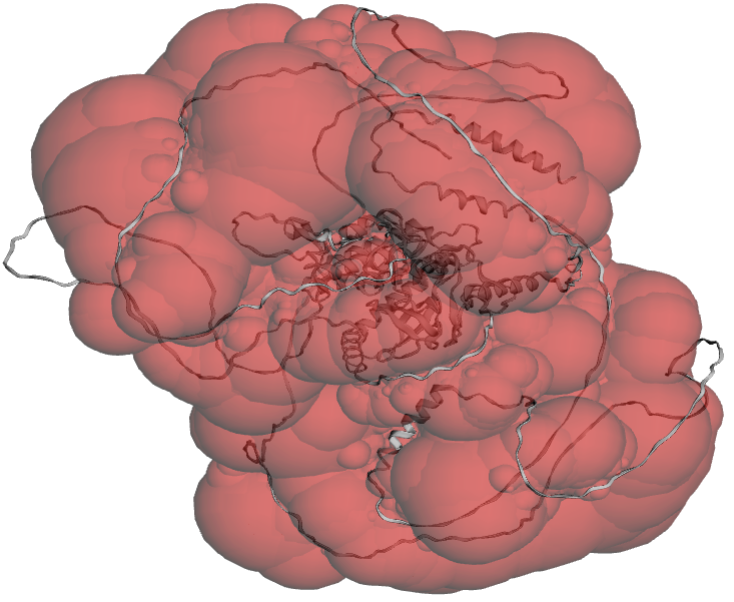
\includegraphics[width=6cm]{imagenes/activo.png}
	\caption{Sitios activos de la proteína hipotética}
	\label{19}
\end{figure}


\begin{figure}[!h]
	\center
	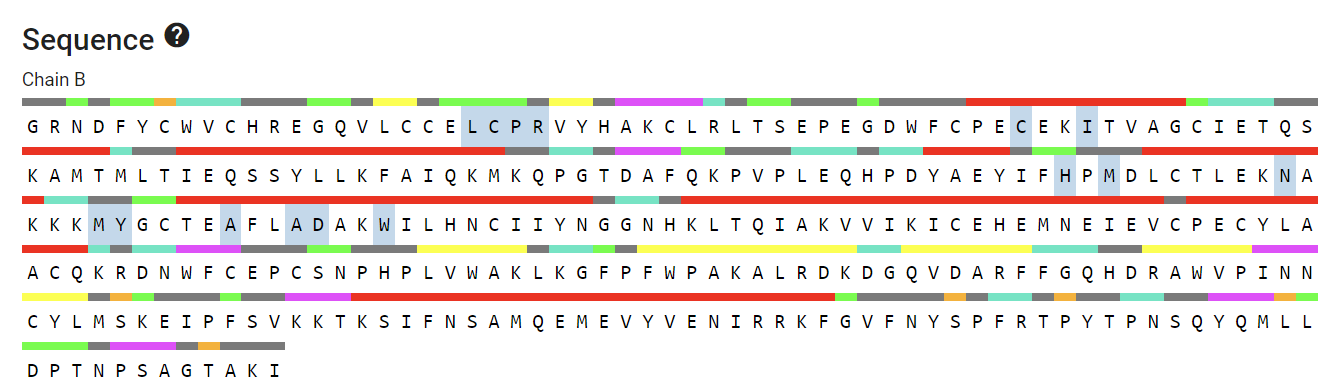
\includegraphics[width=9cm]{imagenes/seq.png}
	\caption{Sitios activos del modelo de Swiss Model de la proteína hipotética. Las esferas rojas representan los sitios activos y los aminoácidos subrayados en gris son los que conforman estos sitios activos.   }
	\label{20}
\end{figure}

Para identificar los sitios activos se usó el modelo generado por Swiss Model, el cual dio el mayor grado de confiabilidad a pesar de representar el 33\% de la proteína hipotética en cuestión. 
En el CASTp se observó que se tiene una zona con sitios activos. Los aminoácidos involucrados en dichos sitios activos son los que están en la Tabla 6.  

\begin{table}[]
	\begin{tabular}{|lllll|}
		\hline
		PocID& Cadena & SeqID  & AA & Átomo \\
	 1&  B&99  & LEU & O \\
	 1&  B& 100 & CYS & CA \\
	 1&  B& 100 & CYS & CB \\
	 1&  B& 101 & PRO & CD \\
	 1&  B& 102 & ARG & NH2 \\
	 1&  B& 124 & CYS & CA \\
	 1&  B& 124 & CYS & SG \\
	 1&  B& 127 & ILE & CB \\
	 1&  B& 127 & ILE & CG2 \\
	 1&  B& 127 & ILE & CD1 \\
	 1&  B& 185 & HIS & CE1 \\
	 1&  B& 185 & HIS & NE2 \\
	 1&  B& 187 & MET & CE \\
	 1&  B& 195 & ASN & ND2 \\
	 1&  B& 200 & MET & O \\
	 1&  B& 200 & MET & CB \\
	 1&  B& 200 & MET & CE \\
	 1&  B& 201 & TYR & CD1 \\
	 1&  B& 201 & TYR & CE1 \\
	 1&  B& 206 & ALA & CA \\
	 1&  B& 206 & ALA & O \\
	 1&  B& 206 & ALA & CB \\
	 1&  B& 209 & ALA & CB \\
	 1&  B& 210 & ASP & CG \\
	 1&  B& 210 & ASP & OD1 \\
	 1&  B& 210 & ASP & OD2 \\
	 1&  B& 213 & TRP & NE1 \\ \hline
	 
	\end{tabular}
	\caption{Aminoácidos constituyentes de los sitios activos. }

	\end{table}
	El sitio activo identificado tiene un área de 127.830 [Ų]  y un volumen de 131.883[ų] .
   \section{Conclusion}
 
   La identificación de funciones proteicas, sobre todo en el genoma humano, es fundamental para el mejor entendimiento de procesos biológicos. Lo que puede tener impactos positivos en aplicaciones biotecnológicas y médicas. Este estudio, enfocado en identificar posibles funciones, conformaciones e interacciones, implementó múltiples herramientas bioinformáticas con las cuales se caracterizó, encontrando varias proteínas homólogas, la proteína hipotética CAI46211.1. Se encontraron funciones de unión para quinasas tipo C, actividad transductora, así como 4 motivos claramente identificados: DUF3544, Bromodominio, PHD, y PWWP.
Adicionalmente, es muy importante resaltar las interacciones entre CAI46211.1 y otras proteínas, particularmente ZMYND8 la cuál es esencial para la proliferación de AML y que se asocia con   potenciadores de MYC y IRF8, esta proteína  ha sido  considerada por múltiples investigaciones como target terapéutico  al modular transcripción  de AML. Siendo estos, factores importantes para tratamientos de leucemia y carcinomas hepatocelulares [2]. 
Finalmente se concluye sobre el interés de esta proteína hipotética en sus posibles repercusiones sobre los estudios de cáncer y se espera que se siga el análisis de esta proteína que podría influenciar los estudios de terapia de cáncer con inhibidores de Bromodominios [2] así como con sus interacciones con otras proteínas fuertemente relacionadas con terapias de cáncer.  


\ifCLASSOPTIONcaptionsoff
  \newpage
\fi


\begin{thebibliography}{1}


 \bibitem{IEEEhowto:Monteria}
 $Cochran, A.G., Conery, A.R. \& Sims, R.J. Bromodomains: a new target class for drug development. Nat Rev Drug Discov 18, 609-628 (2019). https://doi.org/10.1038/s41573-019-0030-7
$
 \bibitem{IEEEhowto:Monteria}
 $Zhendong Cao, Krista A. Budinich, Hua Huang, Kathrin M. Bernt . 2021. ZMYND8-regulated IRF8 transcription axis is an acute myeloid leukemia dependency.  ARTICLE MOLECULAR CELL VOLUME 81, ISSUE 17, P3604-3622.E10, SEPTEMBER 02, 2021- :https://doi.org/10.1016/j.molcel.2021.07.018
$
\end{thebibliography}



\end{document}
